% do not change these two lines (this is a hard requirement
% there is one exception: you might replace oneside by twoside in case you deliver 
% the printed version in the accordant format
\documentclass[11pt,titlepage,oneside,openany]{article}
\usepackage{times}

\usepackage{url}
\usepackage[hidelinks]{hyperref}
\usepackage{graphicx}
\usepackage{latexsym}
\usepackage{amsmath}
\usepackage{amssymb}

\usepackage{ntheorem}

% \usepackage{paralist}
\usepackage{tabularx}

% this packaes are useful for nice algorithms
\usepackage{algorithm}
\usepackage{algorithmic}

% well, when your work is concerned with definitions, proposition and so on, we suggest this
% feel free to add Corrolary, Theorem or whatever you need
\newtheorem{definition}{Definition}
\newtheorem{proposition}{Proposition}


% its always useful to have some shortcuts (some are specific for algorithms
% if you do not like your formating you can change it here (instead of scanning through the whole text)
\renewcommand{\algorithmiccomment}[1]{\ensuremath{\rhd} \textit{#1}}
\def\MYCALL#1#2{{\small\textsc{#1}}(\textup{#2})}
\def\MYSET#1{\scshape{#1}}
\def\MYAND{\textbf{ and }}
\def\MYOR{\textbf{ or }}
\def\MYNOT{\textbf{ not }}
\def\MYTHROW{\textbf{ throw }}
\def\MYBREAK{\textbf{break }}
\def\MYEXCEPT#1{\scshape{#1}}
\def\MYTO{\textbf{ to }}
\def\MYNIL{\textsc{Nil}}
\def\MYUNKNOWN{ unknown }
% simple stuff (not all of this is used in this examples thesis
\def\INT{{\mathcal I}} % interpretation
\def\ONT{{\mathcal O}} % ontology
\def\SEM{{\mathcal S}} % alignment semantic
\def\ALI{{\mathcal A}} % alignment
\def\USE{{\mathcal U}} % set of unsatisfiable entities
\def\CON{{\mathcal C}} % conflict set
\def\DIA{\Delta} % diagnosis
% mups and mips
\def\MUP{{\mathcal M}} % ontology
\def\MIP{{\mathcal M}} % ontology
% distributed and local entities
\newcommand{\cc}[2]{\mathit{#1}\hspace{-1pt} \# \hspace{-1pt} \mathit{#2}}
\newcommand{\cx}[1]{\mathit{#1}}
% complex stuff
\def\MER#1#2#3#4{#1 \cup_{#3}^{#2} #4} % merged ontology
\def\MUPALL#1#2#3#4#5{\textit{MUPS}_{#1}\left(#2, #3, #4, #5\right)} % the set of all mups for some concept
\def\MIPALL#1#2{\textit{MIPS}_{#1}\left(#2\right)} % the set of all mips





\begin{document}

\pagenumbering{roman}
% lets go for the title page, something like this should be okay
\begin{titlepage}
	\vspace*{2cm}
  \begin{center}
   {\Large IE650 Semantic Web Technologies\\}
   \vspace{2cm} 
   {Project Outline\\}
   \vspace{2cm}
   {presented by\\
    Oliver Frendo (1510432) \\
    Sascha Ulbrich (1493181) \\
   }
   \vspace{1cm} 
   {submitted to the\\
    Data and Web Science Group\\
    Prof.\ Dr.\ Paulheim\\
    University of Mannheim\\} \vspace{2cm}
   {October 2016}
  \end{center}
\end{titlepage} 

% no lets make some add some table of contents
%\tableofcontents
%\newpage

%\listofalgorithms

%\listoffigures

%\listoftables

% evntuelly you might add something like this
% \listtheorems{definition}
% \listtheorems{proposition}

\newpage


% okay, start new numbering ... here is where it really starts
\pagenumbering{arabic}

\section{Goal of the application}
The goal of the application is to allow a user browsing websites to
automatically retrieve additional information about entities in a given text. 
As an example a section of text on a news website containing the entities
``SAP\_SE'' and ``Hasso Plattner'' is marked by the user. This is sent to
a server for processing. As a result the user is shown information gathered from
the semantic web about these two entities. There will be a focus on the entity
types Person, Location and Organisation because each of them has
a comparatively obvious set of properties that are interesting to the user.

\section{Datasets}
The underlying dataset used for retrieving information will be
DBpedia. To enable querying and
subsequent display in the Chrome extension another dataset will be created manually.
For example, the DBpedia page for 
\texttt{SAP\_SE}\footnote{See \url{http://dbpedia.org/page/SAP\_SE}} contains
two properties for its website: \texttt{dbp:homepage} and \texttt{foaf:homepage}.
A similar property found on another page is \texttt{dbp:website}. The manually
created dataset would contain three triples:
\begin{center}
\begin{tabular}{lll}
\texttt{swt:homepage} & \texttt{owl:sameAs} & \texttt{dbp:hompage} .   \\
\texttt{swt:homepage} & \texttt{owl:sameAs} & \texttt{dbp:website} .   \\
\texttt{swt:homepage} & \texttt{owl:sameAs} & \texttt{foaf:homepage} .
\end{tabular}
\end{center}

To show the values in the Chrome extension any results from DBpedia and the
manual dataset are first combined via reasoning. A new SPARQL query is then
generated that queries locally for properties of our own schema. For the example
above this would be \texttt{swt:homepage}. The application will focus on
English texts and will prioritize English labels for simplicity.

Optionally, additional datasets such as
Yago\footnote{See \url{http://yago-knowledge.org}} could be used to increase the
amount of available information. The process to use this would be the same: A query is sent to a DBpedia endpoint, to a Yago
endpoint and results are combined with the manual dataset via reasoning. 
However, to avoid the complexity of Web Data Integration, we treat the problem
of data fusion as out of scope. If multiple values from different sources are
retrieved for a property we will use simple rules to choose which values are
shown to the user. For example, if there are multiple numbers the maximum is
chosen, i.e. for the number of employees of a company it is assumed that the company will keep on growing.

%For strings
%DBpedia is treated as having a higher provenance and will be used as the
%default. If no values are found in DBpedia, Yago is used. 



\section{Technical architecture}
In general the idea is to use a client which collects the relevant text and
calls a backend to retrieve the requested information. The backend processes the
text information and assembles the result containing the requested information
derived from potentially multiple sources. Figure \ref{fig:architecture}
provides a general overview which is described in more detail in the following
paragraphs.

\paragraph{Client.}
We plan to use a Chrome extension for integration with a browser, so the
end user gets the information right away during browsing without a tool change.
The Chrome extension will connect to a Java server via a REST API and will send
the text as well as the requested properties. Only properties defined in our own
schema are allowed. If we manage to maintain a sufficient amount of properties,
an additional feature for the Chrome extension could be to allow the user to
customize the subset of properties per entity type.

\paragraph{Backend.}
For the backend we plan to use Heroku\footnote{See
\url{https://www.heroku.com/}} as platform for hosting a Java server. One reason
is that Heroku offers support for HTTPS which is important to allow the chrome
extension to work on HTTPS websites as well. 
The backend first needs to analyze the text which is done by a component
performing Named Entity Recognition (NER), e.g. Stanford CoreNLP\footnote{See
\url{http://nlp.stanford.edu/software/CRF-NER.shtml}} which runs on Java. After
identifying the named entities Jena\footnote{See \url{https://jena.apache.org/}}
is used locally to query the requested properties of the entity types via SPARQL
from a model consisting of multiple sources, which means a model union is
performed.
Furthermore the backend will offer a REST service providing the list of
available properties per entity type.

\paragraph{Sources.}
As sources we are going to use DBPedia via its SPARQL endpoint and our own
collection of \texttt{owl:sameAs} relations as described in the previous
section. The unioned model should allow the reasoner to use one property of
our own schema definition and retrieve all variants of it. This should work
across sources as well, meaning we could integrate further datasets like Yago
and add them to the model union. However, we would have to extend our own schema
definition per additional source. 

In a first version the model union will be performed per user query. In a second
iteration we could consider using the TDA storage integrated in
Jena to persist the retrieved and unioned data.

\begin{figure}[ht]
	\centering
	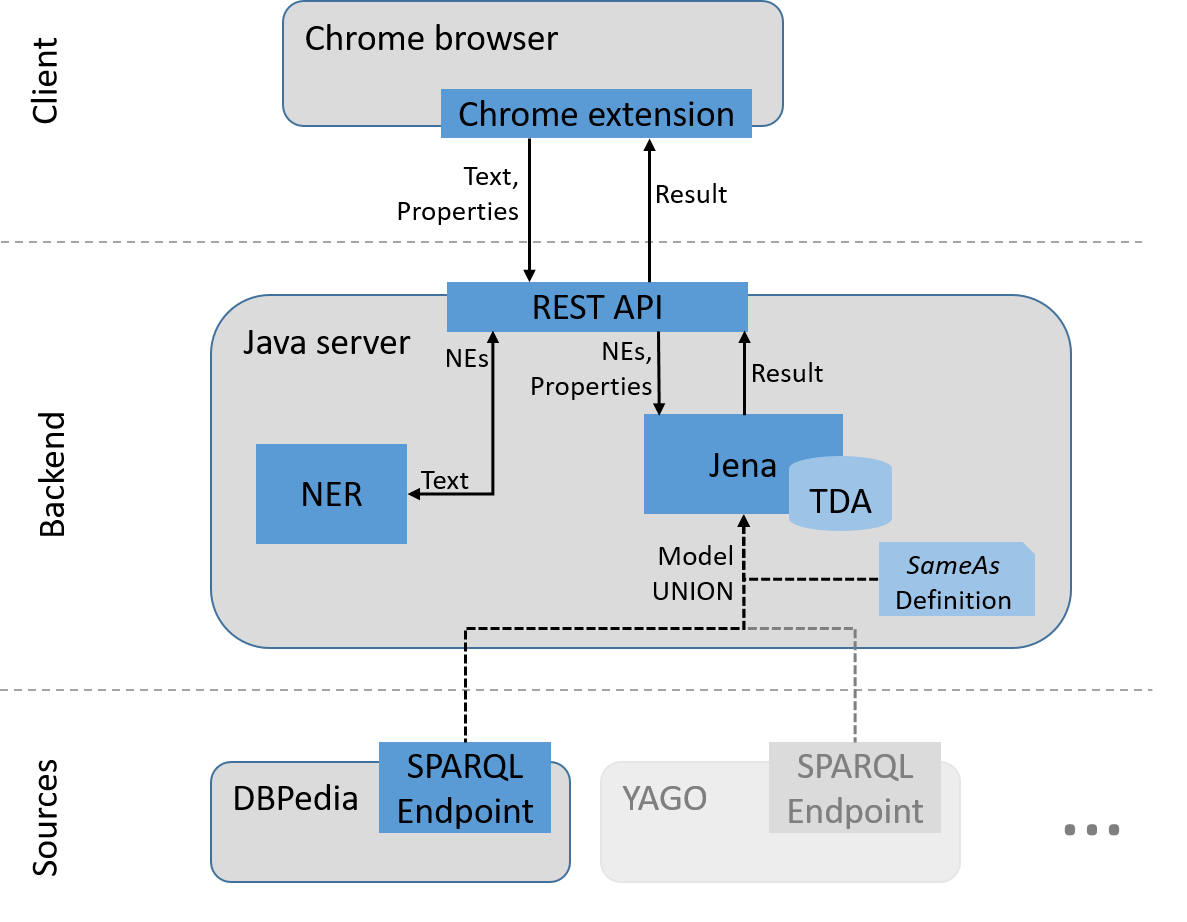
\includegraphics[width=0.8\textwidth]{architecture}
	\caption{Draft of architecture}
	\label{fig:architecture}
\end{figure}


\section{Evaluation}
The application will be evaluated by measuring the recall based on a gold
standard. The gold standard will contain samples of entities and the properties
we aim to retrieve. On the one hand this gives an indication of how good the
application is at retrieving entities itself, which depends on the method and
framework used, i.e. Named Entity Recoginition. On the other hand it also shows
how good our manually created dataset is at combining properties by comparing
which property exists and which property would be shown in the Chrome extension.













\end{document}
